%%%%%%%%%%%%%%%%%%%% book.tex %%%%%%%%%%%%%%%%%%%%%%%%%%%%%
%
% sample root file for the chapters of your "monograph"
%
% Use this file as a template for your own input.
%
%%%%%%%%%%%%%%%% Springer-Verlag %%%%%%%%%%%%%%%%%%%%%%%%%%


% RECOMMENDED %%%%%%%%%%%%%%%%%%%%%%%%%%%%%%%%%%%%%%%%%%%%%%%%%%%
\documentclass[envcountsame,envcountchap]{svmono}
%\documentclass[envcountsame,envcountchap]{svmono}

% choose options for [] as required from the list
% in the Reference Guide, Sect. 2.2

\usepackage{makeidx}         % allows index generation
\usepackage{graphicx}        % standard LaTeX graphics tool
\usepackage{amsmath,amssymb}         % matrices
\usepackage{enumerate}
                             % when including figure files
\usepackage{multicol}        % used for the two-column index
\usepackage[bottom]{footmisc}% places footnotes at page bottom
% etc.
% see the list of further useful packages
% in the Reference Guide, Sects. 2.3, 3.1-3.3


\DeclareMathOperator{\End}{End}
\DeclareMathOperator{\Aut}{Aut}
\DeclareMathOperator{\Hom}{Hom}
\DeclareMathOperator{\support}{supp}


% NEW COMMANDS

%It is standard in Latex to write "macros" which are shorthand for an entire series of instructions. Here are some examples

%Number sets
\newcommand{\N}{\mathbb N}
%So typing \N produces the correct mathematical symbol for the natural numbers
\newcommand{\Z}{\mathbb Z}
\newcommand{\Q}{\mathbb Q}
\newcommand{\R}{\mathbb R}
\newcommand{\C}{\mathbb C}
\newcommand{\K}{\mathbb K}
%notations quelquonques
\newcommand{\tg}[1]{\textbf{#1}}
\newcommand{\ub}[1]{\overline{#1}}

%notations des objets simples
\newcommand{\es}{\emptyset}
\newcommand{\nes}{$\not= \emptyset$}
\newcommand{\sub}{\subset}
\newcommand{\norm}[2]{\lVert #1 \lVert_{#2}}
\newcommand{\vect}[2]{(#1_1,#1_2, \dots, #1_#2)}
\newcommand{\modu}[1]{\lvert#1\lvert}
\newcommand{\B}[3]{B_{#1}\big(#2,#3\big[}
%notations mathématiques
\newcommand{\lb}{\lbrack}
\newcommand{\rb}{\rbrack}
\newcommand{\lv}{\lVert}
%limits and sum
\newcommand{\s}[2]{\sum\limits_{#1}^{#2}}
\newcommand{\li}[2]{\xrightarrow[#1\rightarrow#2]{}}
\newcommand{\lis}[1]{\xrightarrow[n\rightarrow+\infty]{#1}}
\newcommand{\lif}[1]{\xrightharpoonup[n\rightarrow+\infty]{#1}}
\newcommand{\lic}[3]{\xrightarrow[#1\rightarrow#2]{#3}}

\newcommand{\bcup}[2]{\bigcup\limits_{#1}^{#2}}
\newcommand{\bcap}[2]{\bigcap\limits_{#1}^{#2}}

\newcommand{\inv}[1]{\frac{1}{#1}}
\newcommand{\prods}[2]{\langle\qq #1\qq,\qq#2\qq\rangle}

\newcommand{\restr}[2]{#1_{\mkern 2mu \vrule height 2ex\mkern2mu #2} }
\newcommand{\quot}[2]{{\raisebox{.2em}{$#1$}\left/\raisebox{-.2em}{$#2$}\right.}}
\newcommand{\limite}[2]{\underset{#1\rightarrow#2}{\text{lim}}}
\newcommand{\espp}[2]{Ker\big(u-{#1} Id_{#2}\big)}
\newcommand{\fct}[4]{\qq:\qq #1\qq\longrightarrow\qq #2\qq :\qq #3\qq \mapsto\qq #4}

\newcommand{\lam}{\lambda}
\newcommand{\q}{\quad}
\newcommand{\qq}{\text{ }}

\newcommand{\liste}[2]{#1_1, #1_2,..,#1_{#2}}

\newcommand{\maxx}[1]{\underset{#1}{\text{max}}}
\newcommand{\minn}[1]{\underset{#1}{\text{min}}}
\newcommand{\supp}[1]{\underset{#1}{\text{sup}}}
\newcommand{\inff}[1]{\underset{#1}{\text{inf}}}

\newcommand{\fctt}[2]{\qq:\qq#1\qq\rightarrow\qq#2}
\newcommand{\liminff}[1]{\underset{#1\rightarrow+\infty}{\text{liminf}}}
\newcommand{\limsupp}[1]{\underset{#1\rightarrow+\infty}{\text{limsup}}}

\newcommand{\adh}[2]{\text{Adh}_{#1}\big(#2\big)}
\newcommand{\wed}[3]{#1_#2\wedge\dots \wedge #1_#3}


\makeindex             % used for the subject index
                       % please use the style svind.ist with
                       % your makeindex program


%%%%%%%%%%%%%%%%%%%%%%%%%%%%%%%%%%%%%%%%%%%%%%%%%%%%%%%%%%%%%%%%%%%%%

\begin{document}

\author{MATH-F-427 students}
\title{Coxeter groups}
\subtitle{Course notes}
\maketitle

\frontmatter%%%%%%%%%%%%%%%%%%%%%%%%%%%%%%%%%%%%%%%%%%%%%%%%%%%%%%

\tableofcontents

\section{Classification of the Coxeter groups}

Let $(W,S)$ be a Coxeter system and $(m_{ij})$ the associated Coxeter matrix. As discussed above, if $V$ is a real vector space with basis $\{\alpha_1, \ldots , \alpha_n\}$, we can define a symmetric bilinear form as
\begin{equation}
\langle \alpha_i , \alpha_j \rangle = \left \{
\begin{array}{c @{} c}
    &- \cos \left(\frac{\pi}{m_{ij}} \right) \quad \text{if } m_{ij} < + \infty \\
    &-1 \quad ~~~~~~~~~~~~~\text{if } m_{ij} = + \infty \\
\end{array}
\right.
\end{equation} We proved above that $W$ is finite if and only if $\langle ., . \rangle$ is positive definite. 

\begin{definition}
$W$ is irreducible if its Coxeter graph is connected.
\end{definition}

This definition can be understood from the following observation: if $\Gamma = \Gamma_1 \sqcup \Gamma_2$, then $W_\Gamma = W_{\Gamma_1} \times W_{\Gamma_2}$. 

Let us now introduce some basic notations. Take $\{ e_1, \ldots, e_n \}$ be a basis of a vector space $V$. Take $v = \sum_i x_i e_i$ and $w =  \sum_i y_i e_i$ in $V$. Writing $g_{ij} = \langle e_i , e_j \rangle$, we have
\begin{equation}
\begin{split}
\langle v, w \rangle &= \sum_i \sum_j x_i y_j \langle e_i, e_j \rangle \\
&= \sum_i \sum_j x_i y_j g_{ij} \\
&= x^T g y 
\end{split}
\end{equation} where, in the last equality, we used matrix notation. 

\begin{lemma} [Sylvester] 
$\langle ., . \rangle$ is positive definite if and only if all the principal minors of $g$ are positive. 
\end{lemma}
\begin{proof}
The condition is necessary. In fact, taking $v = (v_1, \ldots , v_r , 0, \ldots , 0)$, we have $\langle v, v \rangle = v^T g v$.

The condition is also sufficient. In order to show it, let us proceed by induction on the size of $g$. If $g$ is not positive definite, there must be $2$ negative eigenvalues since the determinant is positive. Let $x \neq 0 \neq y$ be $2$ orthogonal eigenvectors associated to these eigenvalues. Let $\alpha, \beta \in \mathbb{R}$ such that $(\alpha, \beta) \neq (0, 0)$. We write
\begin{equation}
v := \alpha x + \beta y = (*, *, \ldots , * 0 ) \neq 0
\end{equation}   We have
\begin{equation}
v^T g v = \alpha^2 x^T g x + \beta^2 y^T g y \le 0
\end{equation} This implies that that the determinant is non-positive. 
\end{proof}

\begin{theorem}
The irreducible finite Coxeter groups are given in figure \ref{Classification}.
\begin{figure}[h!]
\centering
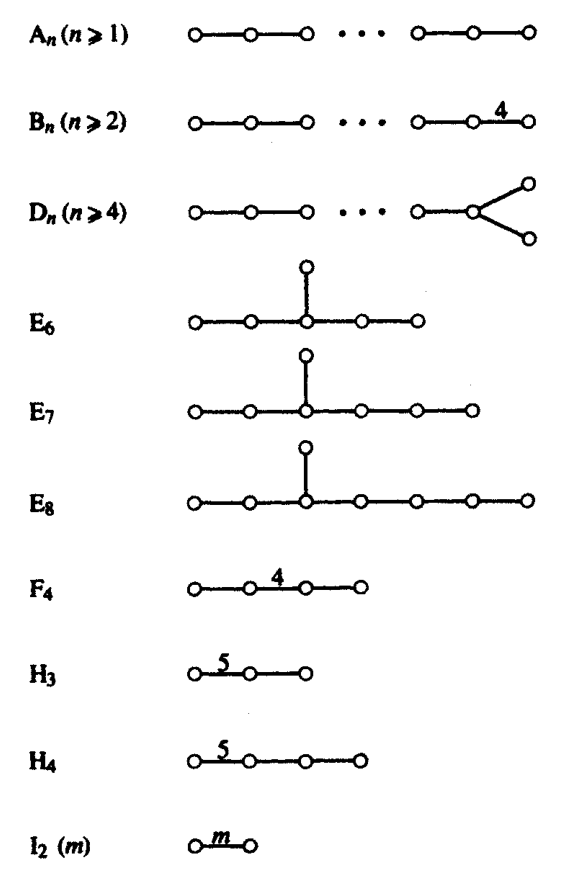
\includegraphics[scale=0.6]{Classification.png}
%\caption{The }
\label{Classification}
\caption{}
\end{figure}    
\label{classification thm}
\end{theorem}

\begin{remark}
Define the matrix $A_\Gamma$ by $[A_\Gamma]_{ij} = 2 \langle \alpha_i , \alpha_j \rangle$ and set $d(\Gamma) = \det (A_\Gamma ) $. We make the following observations:
\begin{itemize}
\item Removing one node in a diagram is equivalent to remove the associated line and column. 
\item If $\Gamma = \Gamma_1 \sqcup \Gamma_2$, then $d(\Gamma ) = d (\Gamma_1). d(\Gamma_2)$.
\end{itemize}
\end{remark}

\begin{lemma}
Let $\Gamma$, $\Gamma '$ and $\Gamma ''$ be as in figure \ref{cours9fig1}.

\begin{figure}[h!]
\centering
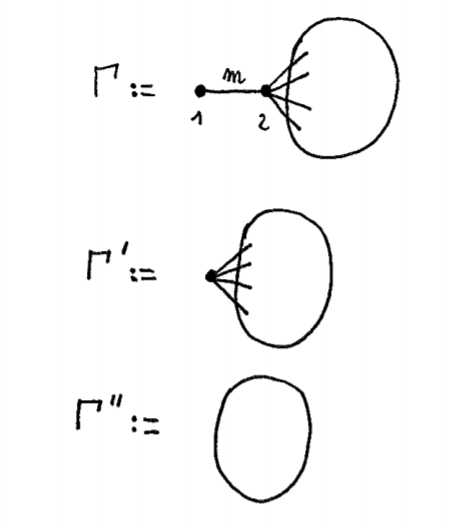
\includegraphics[scale=0.6]{cours9fig1.png}
\caption{}
\label{cours9fig1}
\end{figure}    

Then $d(\Gamma) = 2 d(\Gamma ') - 4 \cos^2 \left(\frac{\pi}{m} \right) d (\Gamma '')$.
\end{lemma}

\begin{proof}
Consider
\begin{equation}
A = \begin{pmatrix}
2 &-\cos \left(\frac{\pi}{m} \right) &0 &\cdots \\
-\cos \left(\frac{\pi}{m} \right) &2 &\cdots & \\
0 &\vdots & 2 &\cdots \\
\vdots &  & \vdots
\end{pmatrix}
\end{equation} We have
\begin{equation}
d (\Gamma ) =2 d(\Gamma ') - (-2) \cos \left(\frac{\pi}{m} \right) (-2) \cos \left(\frac{\pi}{m} \right)  d (\Gamma '')
\end{equation}
\end{proof}

We now compute $d(\Gamma)$ for all the cases in the classification \ref{classification thm}, using the previous lemma. 

\begin{itemize}
\item For the case $A_n$, we have
\begin{equation}
d(A_n) = d(A_{n-1} ) - 4 \cos^2 \left(\frac{\pi}{3} \right) d(A_{n-2}) = n+1
\end{equation} where, to obtain the last equality, we used 
\begin{equation}
d(\circ) =2 \quad \text{and} \quad d(\circ-\circ) = \det \begin{pmatrix}
2 &-1 \\
-1 &2 
\end{pmatrix} = 3
\end{equation}
\item For $B_n$, we have
\begin{equation}
d(B_n) = 2 d(B_{n-1} ) - d (B_{n-2})
\end{equation} for $n\ge 4$, 
\begin{equation}
d(B_3) = 2 d (B_2) - d \circ) = 4-2 = 2 
\end{equation} and
\begin{equation}
d(B_2) = \det \begin{pmatrix}
2 &-2 \cos \left(\frac{\pi}{4} \right) \\
-2 \cos \left( \frac{\pi}{4} \right) & 2 
\end{pmatrix} = 4 - 4 \cos^2 \left( \frac{\pi}{4} \right) = 2
\end{equation} Therefore, $d(B_n) = 2$. 
\item For $D_n$, we have
\begin{equation}
d (D_n) = 2 d(D_{n-1}) - d (D_{n-2})
\end{equation} Furthermore, 
\begin{equation}
\begin{split}
d( {}^\circ_\circ > \circ - \circ ) &= 2 d(  {}^\circ_\circ > ) - d ( {}^\circ_\circ) \\
&= 2 d(A_3) - d (A_1)^2 \\
&= 2 . 4 - 2^2 \\
&= 4
\end{split}
\end{equation} and
\begin{equation}
\begin{split}
d(\circ - \circ - \circ < ^\circ_\circ ) &= 2 d (\circ - \circ < ^\circ_\circ ) - d (\circ < ^\circ_\circ) \\
&= 2 .4 - 4 \\
&= 4 
\end{split}
\end{equation} We deduce that $d(D_n) = 4$. 
\item We proceed in the same way for the other elements the list \ref{classification thm}. We get $d(E_6) = 3$, $d(E_7) = 2$, $d(E_8) = 1$, $d(F_4) = 1$, $d(H_3) = 3 - \sqrt{5} > 0$, $d(H_4) = \frac{7 - 3 \sqrt{5}}{2} > 0$ and $d(I_2 (m) ) = 4 \sin^2 \left( \frac{\pi}{m} \right) > 0$, for $m \ge 3$ ($m= 2$ is disconnected). 

\end{itemize} 

Now, we have to show that there are no other diagrams. In order to do that, le us make some observations.
\begin{itemize}
\item We cannot have diagrams of the type given in figure \ref{cours9fig2}, because there are no relations between these generators. They generate an infinite group. 

\begin{figure}[h!]
\centering
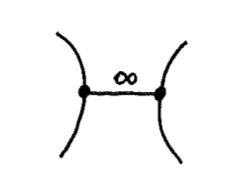
\includegraphics[scale=0.6]{cours9fig2.png}
\caption{}
\label{cours9fig2}
\end{figure}    

\item We cannot have circuits, i.e. diagrams of the type of figure \ref{cours9fig3}


\begin{figure}[h!]
\centering
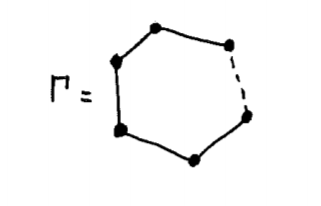
\includegraphics[scale=0.6]{cours9fig3.png}
\caption{}
\label{cours9fig3}
\end{figure}    

In fact, 
\begin{equation}
A_\Gamma = \begin{pmatrix}
2 &* &0 &\cdots &0 &* \\
* &2 &* &0 &\cdots &0 \\ 
0 &* &2 &* &0 &\cdots \\
\vdots & & &\ddots & & \\
0 & & & & &* \\
* &0 &\cdots &0 &* &2
\end{pmatrix}
\end{equation} where
\begin{equation}
\begin{split}
* &= - 2 \cos \left( \frac{\pi}{m} \right) \quad (m\ge 3 ) \\
&\le - 2 \cos \left( \frac{\pi}{3} \right) \\
&-1
\end{split}
\end{equation} Therefore, 
\begin{equation}
\begin{pmatrix}
1 &\cdots &1
\end{pmatrix} A_\Gamma \begin{pmatrix}
1 \\
\vdots \\
1
\end{pmatrix} = 2n + \sum_{\sharp(*) = 2n} (*) \le 2n - 2n = 0
\label{strategy}
\end{equation} and we conclude that $A_\Gamma$ cannot be positive definite.

\item If $\Gamma$ has at most one edge $>3$. In fact, consider a diagram of the type of figure \ref{cours9fig4}.

\begin{figure}[h!]
\centering
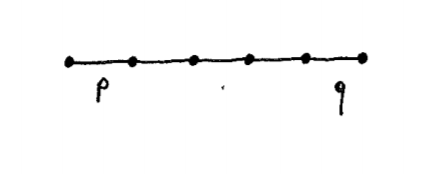
\includegraphics[scale=0.6]{cours9fig4.png}
\caption{}
\label{cours9fig4}
\end{figure}    

\begin{equation}
A_\Gamma = \begin{pmatrix}
2 &-2 \cos \left(\frac{\pi}{p}\right) & & & &\\
-2 \cos \left(\frac{\pi}{p}\right) &2 &-1  & & &\\
 &-1 &2 &-1 & &\\
 & &\ddots &\ddots &\ddots & \\
 & & & & & \\
 & & & & &-2\cos\left(\frac{\pi}{p} \right) \\
 & & & &-2 \cos\left(\frac{\pi}{q} \right) &2 
\end{pmatrix}
\end{equation} We have
\begin{equation}
\begin{split}
d(A_\Gamma ) &= 2 d(B_{n-1} ) - 4 \cos^2 \left( \frac{\pi}{q} \right) d(B_{n-2} ) \\
&= 4 - 8 \cos^2 \left( \frac{\pi}{q} \right) \\
&\le 0 
\end{split}
\end{equation} for $q \ge 4$. The case $q\le 4$ can be done using the same strategy as in \eqref{strategy} and is let as an exercise. 

\item If $\Gamma$ has one edge $> 3$, then $\Gamma$ is a straight line. Consider a diagram of the type of figure \ref{cours9fig5}.

\begin{figure}[h!]
\centering
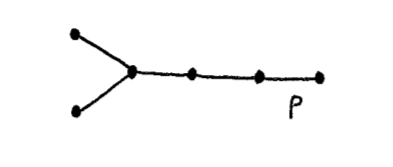
\includegraphics[scale=0.6]{cours9fig5.png}
\caption{}
\label{cours9fig5}
\end{figure}    

\begin{equation}
\begin{split}
d(\Gamma ) &= 2 d(\Gamma_{n-1}) - 4 \cos^2 \left( \frac{\pi}{p} \right) d (D_{n-2}) \\
&= 8 - 16 \cos^2 \left( \frac{\pi}{p} \right) \le 0 \\ 
&\le 0
\end{split}
\end{equation} 

\item $\Gamma$ has at most one branching point. In fact consider a diagram of the type of figure \ref{cours9fig6}.

\begin{figure}[h!]
\centering
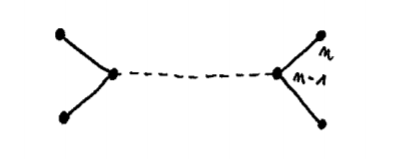
\includegraphics[scale=0.6]{cours9fig6.png}
\caption{}
\label{cours9fig6}
\end{figure}    

We have
\begin{equation}
d(\Gamma) = 2 d(\D_{n-1})) - d (D_{n-3} \cup A_1 ) = 8 - 2.4 = 0
\end{equation}

\item $\Gamma$ has no branching point with $4$ or more branches. In fact,
\begin{equation}
\begin{split}
d(>\circ < ) &= 2 d (>\circ - ) - d ({}_\circ^\circ \circ) \\
&= 2 . 4 - 2^3 \\
&=0
\end{split}
\end{equation}

\item It is let as an exercise to show the relations in figure \ref{cours9fig7}.

\begin{figure}[h!]
\centering
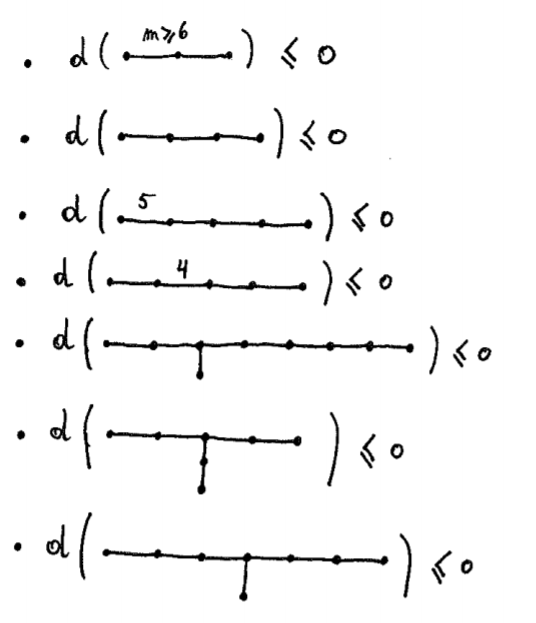
\includegraphics[scale=0.6]{cours9fig7.png}
\caption{}
\label{cours9fig7}
\end{figure}    

Therefore, we conclude that no other diagrams than those identified in theorem \ref{classification thm} are valid.   




 

\end{itemize}








\mainmatter%%%%%%%%%%%%%%%%%%%%%%%%%%%%%%%%%%%%%%%%%%%%%%%%%%%%%%%


	
\end{document}	